\documentclass[12pt,a4paper]{article}
\usepackage{fontspec, xunicode, xltxtra}
\XeTeXlinebreaklocale "zh"
\XeTeXlinebreakskip = 0.1pt plus 1pt minus 0.1pt
\usepackage{xeCJK} 
\usepackage{fontspec}  
\setCJKmainfont{SimSun} 
\setCJKmonofont{SimSun} 
\setmainfont{Courier}%{Times New Roman} {SourceCodePro-Regular}{Consolas}{Courier}
\usepackage{indentfirst} 
\setlength{\parindent}{2em}
\usepackage{float}
\usepackage[utf8]{inputenc}
\usepackage{setspace}
\usepackage[colorlinks,linkcolor=black,anchorcolor=black,citecolor=black]{hyperref}
\usepackage{amsmath}
\usepackage{amsfonts}
\usepackage{amssymb}
\usepackage{geometry}
\geometry{left=2.5cm,right=2.5cm,top=2.5cm,bottom=4cm}
\usepackage{listings}
\lstset{language=C++}
\lstset{breaklines}
\lstset{extendedchars=false}
\usepackage{fancyhdr}
\pagestyle{fancy}
\lhead{数据结构大作业报告}
\author{姚皓天(2013011515)}
\title{数据结构大作业报告\\\ \\ 图数据结构与路径规划的应用\\ Rev 1.0}
\date{2015年1月}
\graphicspath{{Figure/}}
\begin{document}
\maketitle
\thispagestyle{empty}
\newpage
初步文档,稍后完善。
\newpage
\thispagestyle{empty}
\renewcommand\contentsname{\textbf{目录}}
\tableofcontents
\newpage
\section{基本原理}
\subsection{概述}
本程序是由 Microsoft Visual Studio 2012 创建,目标框架为 .NET Framework 4.5 ,WPF应用程序。
程序第一部分实现了图结构的存储,遍历,多元最短路的规划,以及相应的可视化操作;第二部分使用蚁群算法(和并行文件查找遍历)的路线推荐功能。
\subsection{原理}
命名空间TravelAgency.Graph下实现了城市类和图类的数据结构的封装,实现了图的存储,修改,遍历等基本操作,以及对Floyd算法。\par
命名空间TravelAgency.ACO下实现了蚁群算法。\par
命名空间TravelAgency下实现了基本的界面交互逻辑以及文件操作。
\subsection{界面}
\begin{figure}[H]
\centering
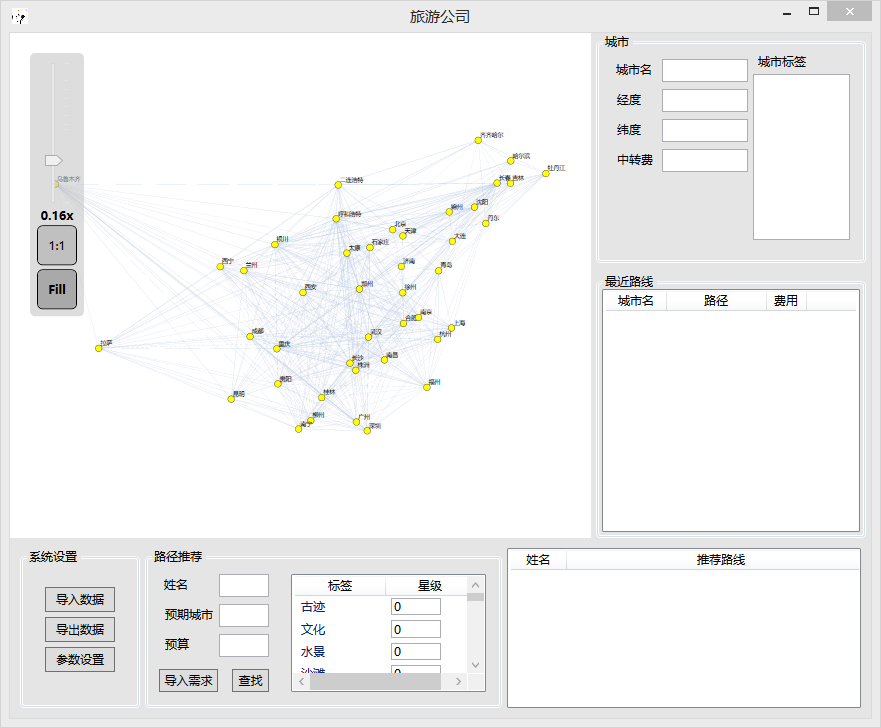
\includegraphics[width=0.6\textwidth]{1.png}
\caption{主界面} 
\end{figure}
\begin{figure}[H]
\centering
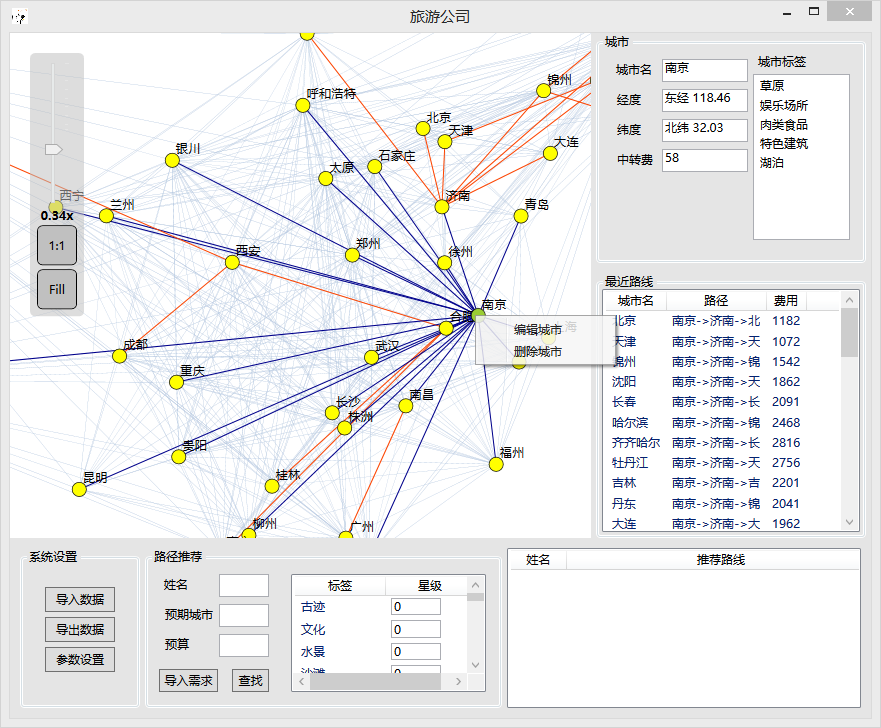
\includegraphics[width=0.6\textwidth]{2.png}
\caption{修改删除节点} 
\end{figure}
\begin{figure}[H]
\centering
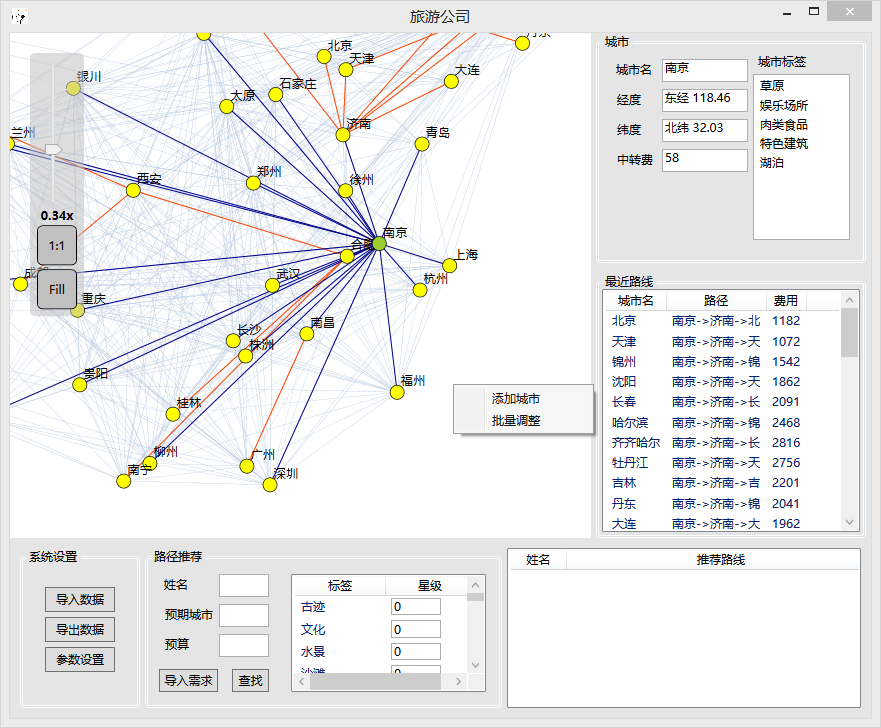
\includegraphics[width=0.6\textwidth]{3.png}
\caption{添加节点} 
\end{figure}
\begin{figure}[H]
\centering
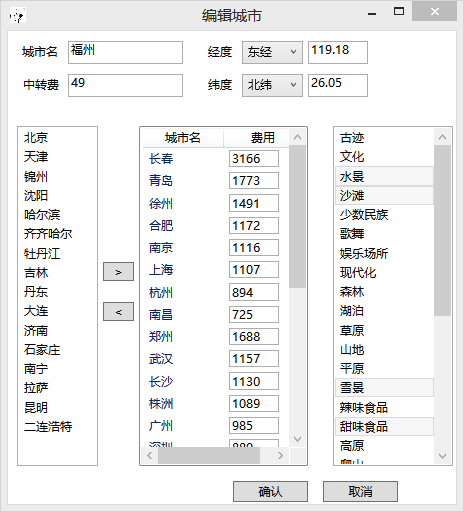
\includegraphics[width=0.6\textwidth]{4.png}
\caption{编辑节点} 
\end{figure}
\begin{figure}[H]
\centering
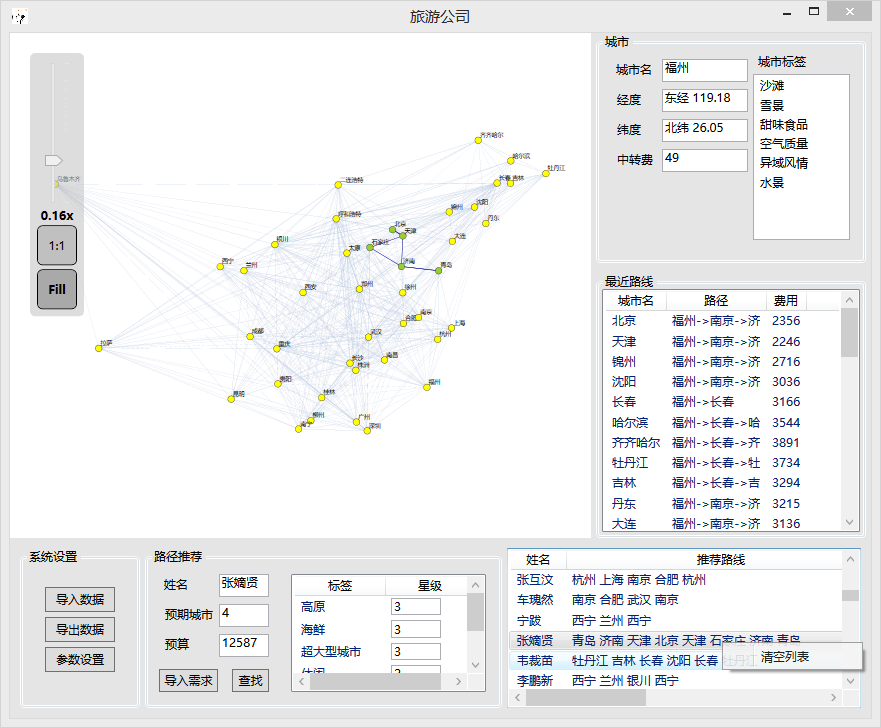
\includegraphics[width=0.6\textwidth]{5.png}
\caption{路径推荐} 
\end{figure}
\subsection{操作说明}
\subsubsection{系统设置}
导入按钮,可以从Excel文件或者地图二进制文件(.map文件)中导入地图信息。导出按钮,可以将地图数据导出到二进制文件中。参数设置可以调整推荐算法的参数。
\subsubsection{缩放}
地图区域提供缩放控件,可以使用缩放功能实现对地图的调整。
\subsubsection{添加节点}
在空白处点击右键可以打开上下文菜单,将弹出添加节点的对话框。对话框初始经纬度就是鼠标点击位置对应的地理坐标。
\subsubsection{修改、删除节点}
右键点击城市,上下文菜单提供修改和删除的选项。
\subsubsection{修改城市}
修改城市信息将在弹出的对话框中完成,对话框中可以添加路径,维护城市标签。
\subsubsection{最短路径}
点击城市,将显示出到达其他所有城市的最优路径,并且直达和非直达路径使用不同的颜色标出。点击城市的同时,右侧将列出城市的详细信息。在右侧路径列表中双击路径,对应的路径将在地图中高亮。
\subsubsection{路线推荐}
在下方填入需求,将会给出推荐路径,双击路径,对应的路径将在地图中高亮。同时在路径列表中右键可以将列表清空。
\section{程序设计}
\subsection{总体框架}
\begin{figure}[H]
\centering
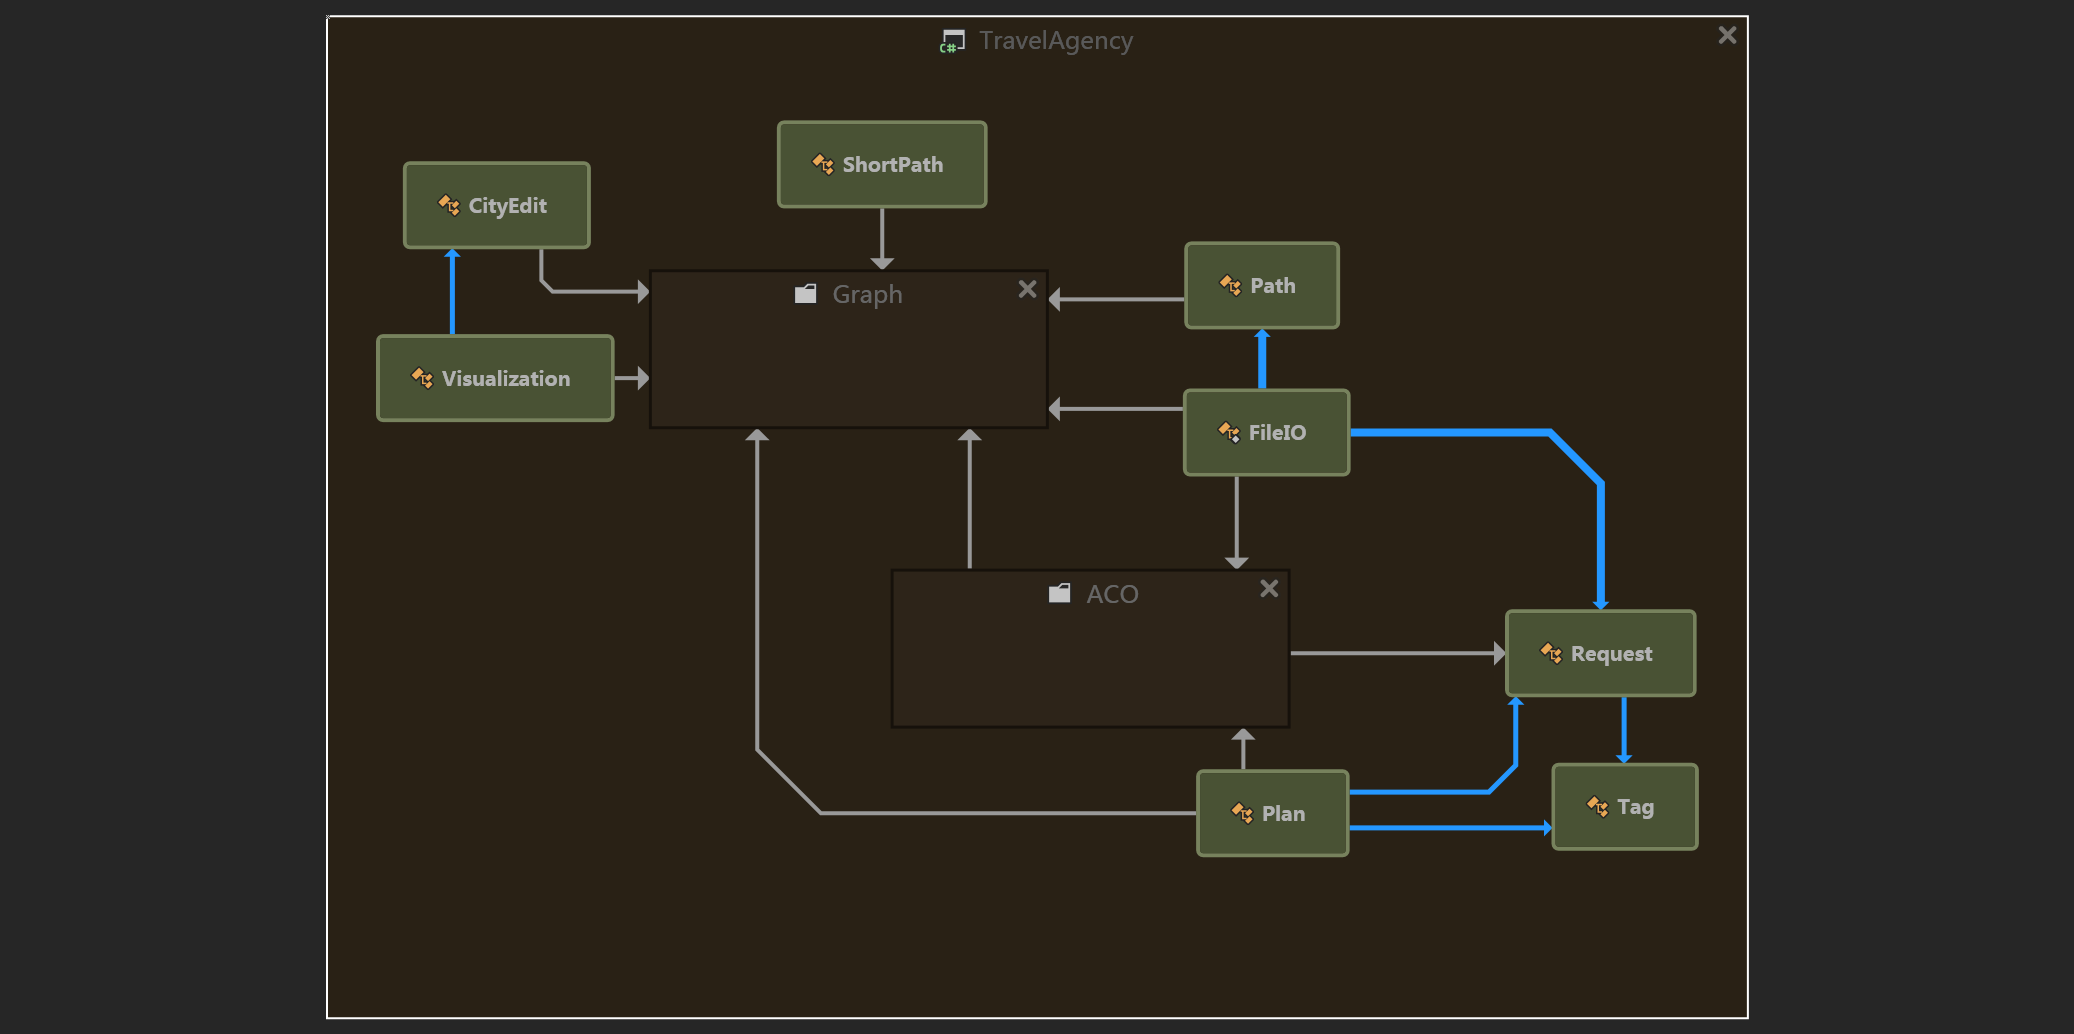
\includegraphics[width=0.8\textwidth]{8.png}
\caption{总体框架} 
\end{figure}
\subsection{图数据结构的实现}
各类的依赖关系如下图:
\begin{figure}[H]
\centering
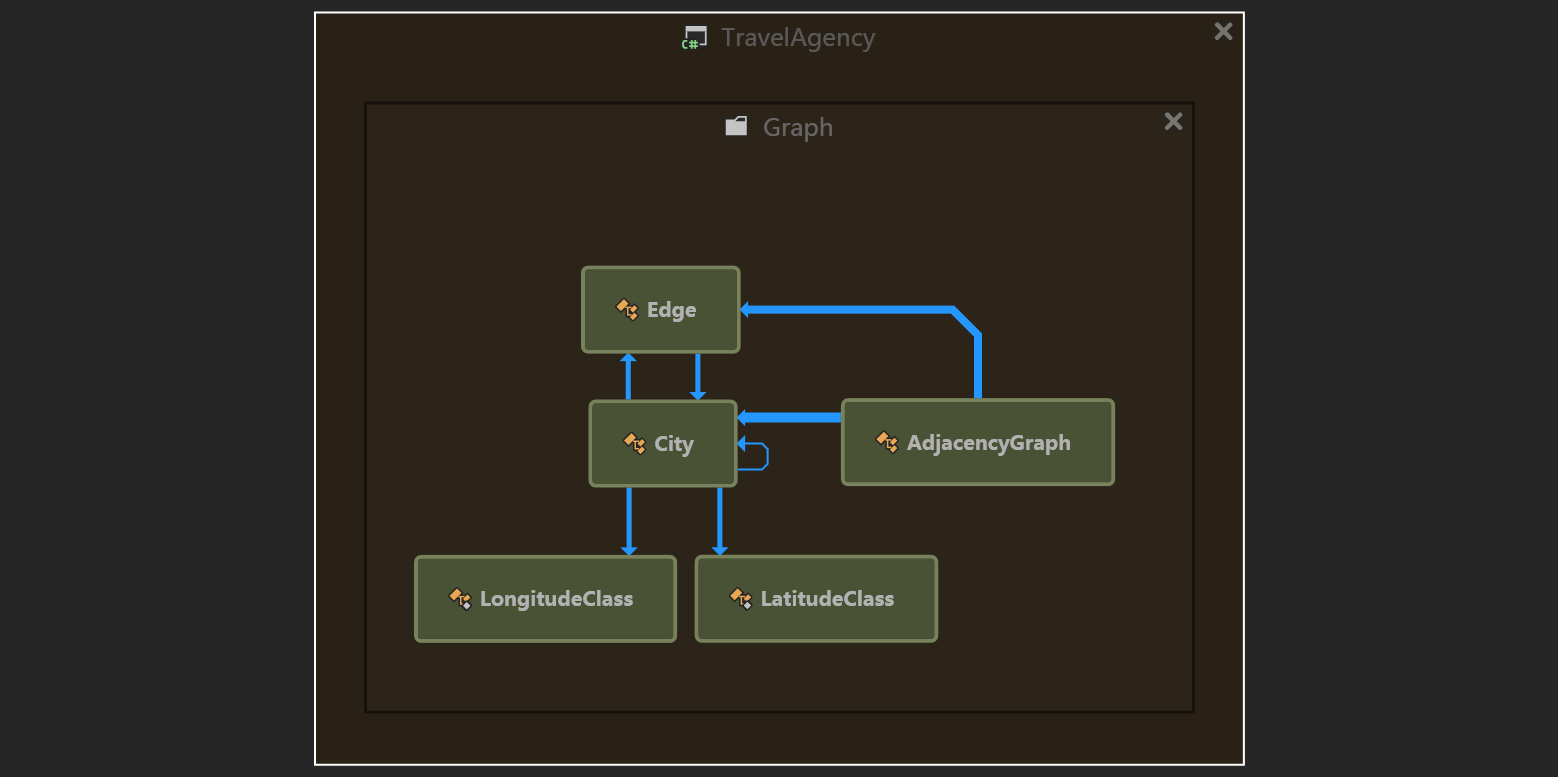
\includegraphics[width=0.8\textwidth]{6.png}
\caption{图类依赖关系} 
\end{figure}
\subsection{最短路径算法}
城市间最短路径的计算采用了Floyd算法。
\subsection{路径推荐算法}
\subsubsection{并行文件查找}
在路径推荐过程中,我首先使用了遍历的方法,遍历所有可能的路径,并将每条路径,具有的标签和总费用保存在文件中。文件按照一定的大小分成区块。得到的一系列路径文件保存在以出发城市名的文件夹中。\par
当用户输入需求的时候,将采用并行的方式,对每个区块的进行处理。计算评估函数的值,最后进行归并,找出最优值。\par
但是由于城市数量较多,在路径长度大于5的情况下,将会有大量的文件需要处理,运算时间过长。
\subsubsection{蚁群算法}
参考文章\url{http://blog.sina.com.cn/s/blog_6a409d870101lwr8.html}\par
实现了蚁群算法,可以较快的给出较优的解。\par
但是由于算法的固有特点,每次所得路径可能会不一致,并且不能保证取到最优解。
各类的依赖关系如下图:
\begin{figure}[H]
\centering
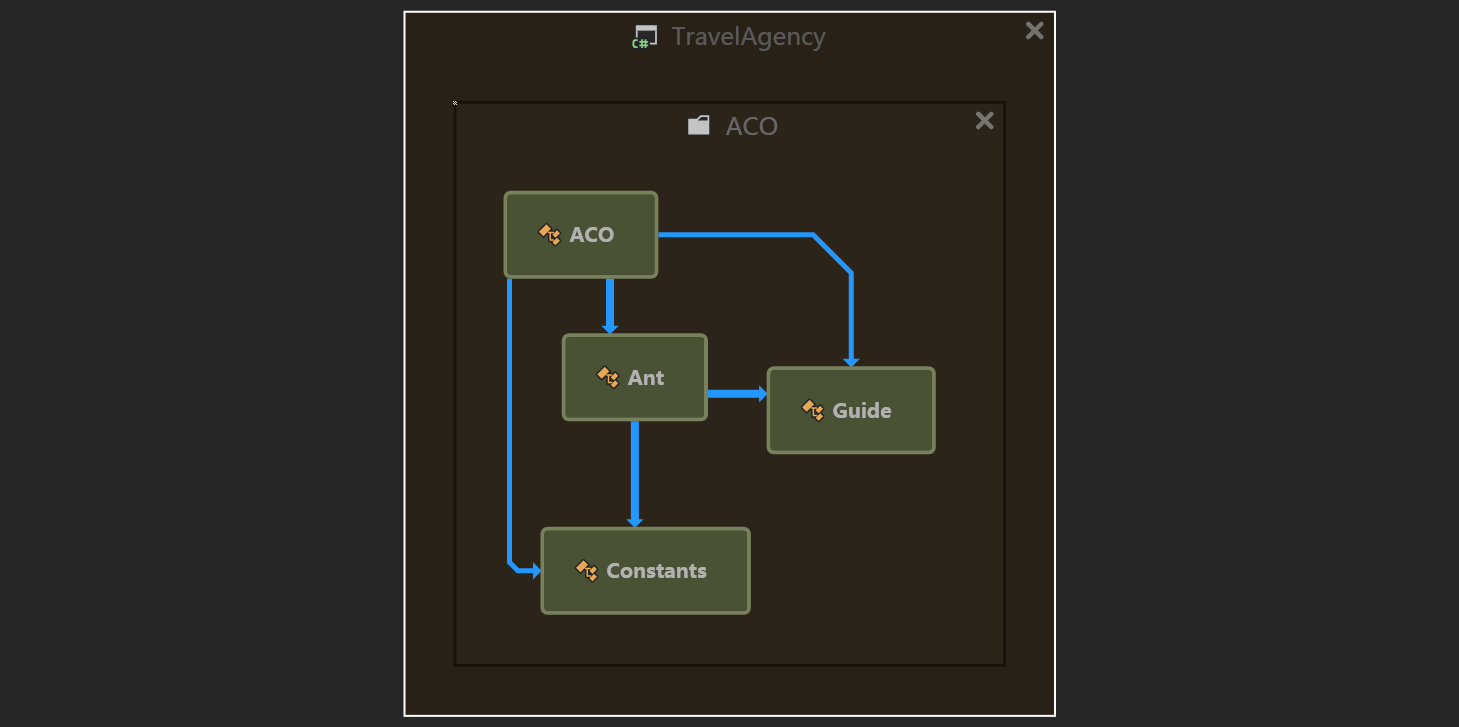
\includegraphics[width=0.8\textwidth]{7.png}
\caption{蚁群算法类依赖关系} 
\end{figure}
\section{设计心得}
\subsection{收获}
这次熟悉了WPF框架下的界面开发,体验了一个较复杂程序的开发。
\section{文件清单}
\begin{itemize}
\item src$\backslash$ 工程文件
\item bin$\backslash$ 可执行文件
\item doc$\backslash$ 文档
\end{itemize}
%程序版本库:\url{https://github.com/yht1995/RBTree.git}
\end{document}